%!TEX root = /Users/nataf/test/DOC/freefem++doc.tex

\subsection{PETSc and HPDDM solvers}


\begin{example}[elasticity-3d.edp]
	A three dimensional elasticity problem is defined. The solver can be either a  domain decomposition method, a direct solver or an algebraic multigrid method. The last two solvers are available via the PETSc~\cite{petsc-efficient,petsc-web-page} interface. Details are given below. 
\end{example}

\def\parallelScript{elasticity-3d.edp}


\subsubsection{Three dimensional elasticity problem} % (fold)
\label{sub:three_dimensional_elasticity_problem}

%\paragraph{Physics of the problem} % (fold)
%\label{par:physics_of_the_problem}

The mechanical properties of a solid can be characterized by its Young modulus $E$ and Poisson ratio $\nu$ or alternatively by its Lam\'e coefficients $\lambda$ and $\mu$. These coefficients relate to each other by the following formulas:
\begin{equation}
	\label{eq:parallel:lambdanu}
\lambda = \frac{E \nu}{(1+\nu) (1- 2 \nu)}\ \text{ and } \ \mu = \frac{E}{2(1+\nu)}\,.
\end{equation}

The reference geometry of the solid is the open $\Omega\subset \R^3$. The solid is subjected to a volume force $\mathbf{f}$ and on part of its boundary ($\Gamma_3$) to a normal stress $\mathbf{g}$. It is clamped on the other part of its boundary  ($\Gamma_1$). Let $\mathbf{u}:\Omega\rightarrow \R^3$ denote the displacement of the solid. In Cartesian coordinates $(x_1,x_2,x_3)$, the linearized strain tensor $\varepsilon({\mathbf{u}})$ is given by:
\[
\epsilon_{ij} (\mathbf{u}) :=  \frac{1}{2} \left( \frac{\partial u_i}{\partial x_j} + \frac{\partial u_j}{\partial x_i}\right) \,, \text{ for }1\le i,j\le 3\,. 
\]
The inner product of two strain-tensors is defined by:
\[
\epsilon (\mathbf{u}) : \epsilon(\mathbf{v}) := \sum_{i=1}^3 \sum_{j=1}^3 \epsilon_{ij} (\mathbf{u})  \epsilon_{ij} (\mathbf{v})\,.
\]
The divergence of the displacement is defined by
\[
\nabla \cdot \mathbf{u} := \sum_{i=1}^3 \frac{\partial u_i}{\partial x_i}\,.
\]

The finite element approximation of the system of linear elasticity is defined by a variational formulation:\\
Find a displacement $\mathbf{u}:\Omega\rightarrow \R^3$ in ${\mathbb P}_2$ so that for any test function $\mathbf{v}:\Omega\rightarrow \R^3$  in ${\mathbb P}_2$, we have:
\begin{align}
\label{eq:linear_elasticity}
a(\mathbf{u}, \mathbf{v}) &\ds := \int_\Omega \lambda\, \nabla \cdot \mathbf{u}\ \nabla \cdot \mathbf{v} + \mu\, \varepsilon(\mathbf{u}) : \varepsilon(\mathbf{v}) 
%\\ &
\ds - \int_\Omega \mathbf{f} \cdot \mathbf{v} = 0\,,
\end{align}
where
\begin{itemize}
\item where $\lambda$ and $\nu$ are defined by formula~\eqref{eq:parallel:lambdanu} Young's modulus $E$ and Poisson's ratio $\nu$ vary between two sets of values, $(E_1, \nu_1) = (2 \cdot 10^{11}, 0.25)$, and $(E_2, \nu_2) = (10^7, 0.45)$.
\item $\mathbf{f}$ are the body forces, in this case only the gravity. 
\end{itemize}
In the FreeFem++ script, equation~\eqref{eq:linear_elasticity} corresponds to three parametrized macros: {\tt epsilon}, {\tt div} and {\tt Varf}. \asupprimer{Pierre : expliquer la notation u\#B} 
\lstinput[linerange=problemPhysics-problemPhysicsEnd]{./PARALLEL/FreefemProgram/\parallelScript}
\vspace{0.5cm}

%\paragraph{Geometry} % (fold)
%\label{par:geometry}
A first geometry is defined via a three dimensional mesh of a (simplified) bridge that is built in two steps:
\begin{itemize}
	\item the mesh of a two dimensional bridge is built {\tt ThGlobal2d}. 
	\item a third dimension is added to the previous 2D mesh using the {\tt buildlayers} function.
\end{itemize}
Note that the three dimensional mesh is not actually built but a macro is defined. 
\lstinput[linerange=sequentialMesh-sequentialMeshEnd]{./PARALLEL/FreefemProgram/\parallelScript}
This geometry is partitioned and distributed among the MPI processes.
\begin{figure}
\centering
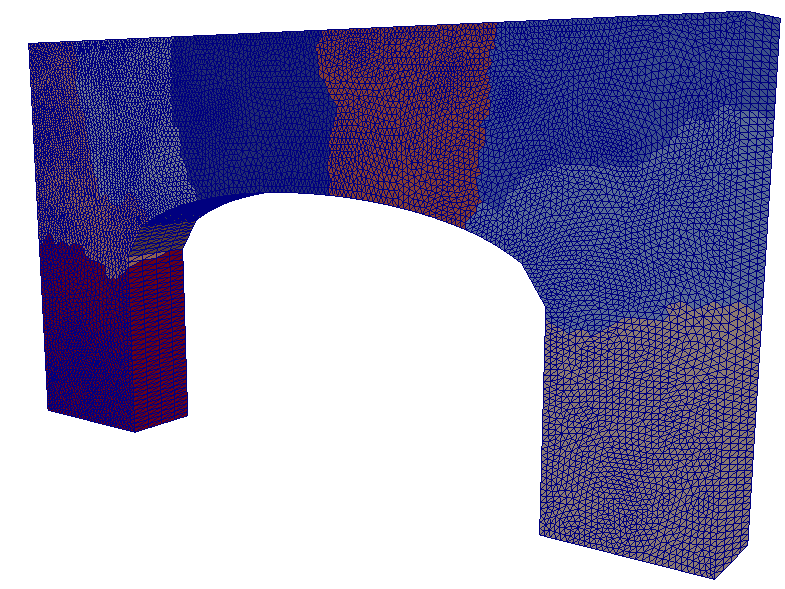
\includegraphics[width=.4\textwidth]{PARALLEL/part.png}
\caption[]{Partitioning into eight subdomains}
\end{figure}
From now on, all the tasks can be computed concurrently, meaning that each MPI process is in charge of only one subdomain and variables are local to each process. Then a parallel mesh refinement is made by cutting each tetrahedra into $8$ tetrahedra. This corresponds to a mesh refinement factor $s$ equals to $2$. Note also that at this point, the displacement field $\mathbf{u}$ is approximated by ${\mathbb P}_2$ continuous piecewise quadratic functions.
\lstinput[linerange=parallelMesh-parallelMeshEnd]{./PARALLEL/FreefemProgram/\parallelScript}



%\paragraph{Physical parameters} % (fold)
%\label{par:physical_parameters}
The Young and Poisson modulus are heterogeneous and the exterior forces are constant.
\begin{remark}
In our numerical experiments, Poisson's ratio being relatively far from the incompressible limit of 0.5, it is not necessary to switch to a mixed finite element formulation since there is no locking effect. 
\end{remark}
\lstinput[linerange=physicalParameters-physicalParametersEnd]{./PARALLEL/FreefemProgram/\parallelScript}
% paragraph physical_parameters (end)



% subsection three_dimensional_elasticity_problem (end)

\subsubsection{Native DDM solvers and PETSc Interface} % (fold)
\label{sub:ddm_solvers_and_petsc_interface}
At this point, the physics, the geometry and the discretization of the three dimensional elasticity problem have been given in the script. In order to find the finite element approximation of the displacement field, we have to solve the corresponding global algebraic system which is actually never assembled. Its distributed storage among the processes depends on whether we use native FreeFem++ solvers or other solvers via the PETSc interface. The native FreeFem++ solvers are:
	\begin{itemize}
		\item a parallel GMRES solver which is the default parallel solver in FreeFem++,
		\item a one-level Schwarz method, either ASM or RAS,
		\item the two-level Schwarz method with a \geneo coarse space, \cite{Dolean:2015:IDD}.
	\end{itemize}
 They are implemented inside HPDDM, a C++ framework for high-performance domain decomposition methods, available at the following URL: \url{https://github.com/hpddm/hpddm}, \cite{Jolivet:2014:HPD}. Its interface with FreeFem++ also include substructuring methods, like the FETI and BDD methods.
 The solvers interfaced with PETSc are:
	\begin{itemize}
		\item the PETSc parallel GMRES solver,
		\item the multi frontal parallel solver MUMPS. %\cite{Amestoy:2001:FAM},
        \item GAMG: an algebraic multigrid solver
% \cite{adams2004ultra}.
	\end{itemize}
\lstinput[linerange=chooseSolver-chooseSolverEnd]{./PARALLEL/FreefemProgram/\parallelScript}

\paragraph{FreeFem++ interface} % (fold)
\label{par:_tt_freefem_interface}


If the native FreeFem++ solvers are used, the local stiffness matrices are assembled concurrently:
\lstinput[linerange=localMatrix-localMatrixEnd]{./PARALLEL/FreefemProgram/\parallelScript}
The local operator is attached to a distributed structure \texttt{dschwarz} which is a FreeFem++ type. If necessary, the \geneo coarse space is built : 
\lstinput[linerange=coarseSpace-coarseSpaceEnd]{./PARALLEL/FreefemProgram/\parallelScript}
The distributed linear system is solved by a call that includes additional command line arguments that are automatically passed to the solvers.
\lstinput[linerange=SolverDDM-SolverDDMEnd]{./PARALLEL/FreefemProgram/\parallelScript}

% paragraph _tt_freefem_interface (end)


\paragraph{PETSc interface} % (fold)
\label{par:_tt_petsc_interface}

If the PETSc interface is used, the local stiffness matrix $K := A_{ii} := R_i A R_i^T$ and the local load vector $rhs$ are built concurrently from the variational forms for all subdomains $1\le i\le N$.
\lstinput[linerange=StiffnessRhsMatrix-StiffnessRhsMatrixEnd]{./PARALLEL/FreefemProgram/\parallelScript}
\texttt{dmatrix} is a FreeFem++ type.

If an algebraic multigrid method is used via the PETSc interface, the near null space must be provided in order to enhance the convergence
%, see e.g. \cite{henson2002boomeramg}
. For an elasticity problem, it is made of the rigid body motions which are three translations and three rotations, here along the axis. 
\lstinput[linerange=rigidBodyMotion-rigidBodyMotionEnd]{./PARALLEL/FreefemProgram/\parallelScript}

Eventually, the solver may be called by passing command line parameters to PETSc:
\lstinput[linerange=SolverPETSc-SolverPETScEnd]{./PARALLEL/FreefemProgram/\parallelScript}

% paragraph _tt_petsc_interface (end)


% subsection ddm_solvers_and_petsc_interface (end)

\subsubsection{Validation of the computation} % (fold)
\label{sub:validation_of_the_computation}
The true residual is computed by first performing a parallel matrix vector product either via matrix {\tt Mat} that is interfaced with the PETSc interface
\lstinput[linerange=matrixVectorPETSc-matrixVectorPETScEnd]{./PARALLEL/FreefemProgram/\parallelScript}
or via the matrix {\tt Aglob} in the ``native'' FreeFem++ Schwarz format.
\lstinput[linerange=matrixVectorFFpp-matrixVectorFFppEnd]{./PARALLEL/FreefemProgram/\parallelScript}


Once the linear system is solved and the residual is computed, the sequel of the program does not depend on whether a FreeFem++ or a PETSc interface was used. 
The residual is subtracted from the distributed right-hand side {\tt rhs}. Then distributed scalar product are performed using  partition of unity matrices $(D_i)_{1\le i \le N}$ where $N$ is the number of subdomains:
\[
\text{dscalprod}(D,U,V) := \sum_{i=1}^N D_i U_i V_i\,.
\]
\lstinput[linerange=trueResidual-trueResidualEnd]{./PARALLEL/FreefemProgram/\parallelScript}
The three dimensional solution can be visualized by the {\tt plot} command. 
\lstinput[linerange=Visualization-VisualizationEnd]{./PARALLEL/FreefemProgram/\parallelScript}

% subsection validation_of_the_computation (end)





% section a_parallel_script (end)


